\thispagestyle{lichsutoanhocnone}
\pagestyle{lichsutoanhoc}
\graphicspath{{../lichsutoanhoc/pic2/}}
\everymath{\color{lichsutoanhoc}}
\blfootnote{$^1$\color{lichsutoanhoc}THPT chuyên Hà Nội -- Amsterdam.}
\begingroup
\AddToShipoutPicture*{\put(0,616){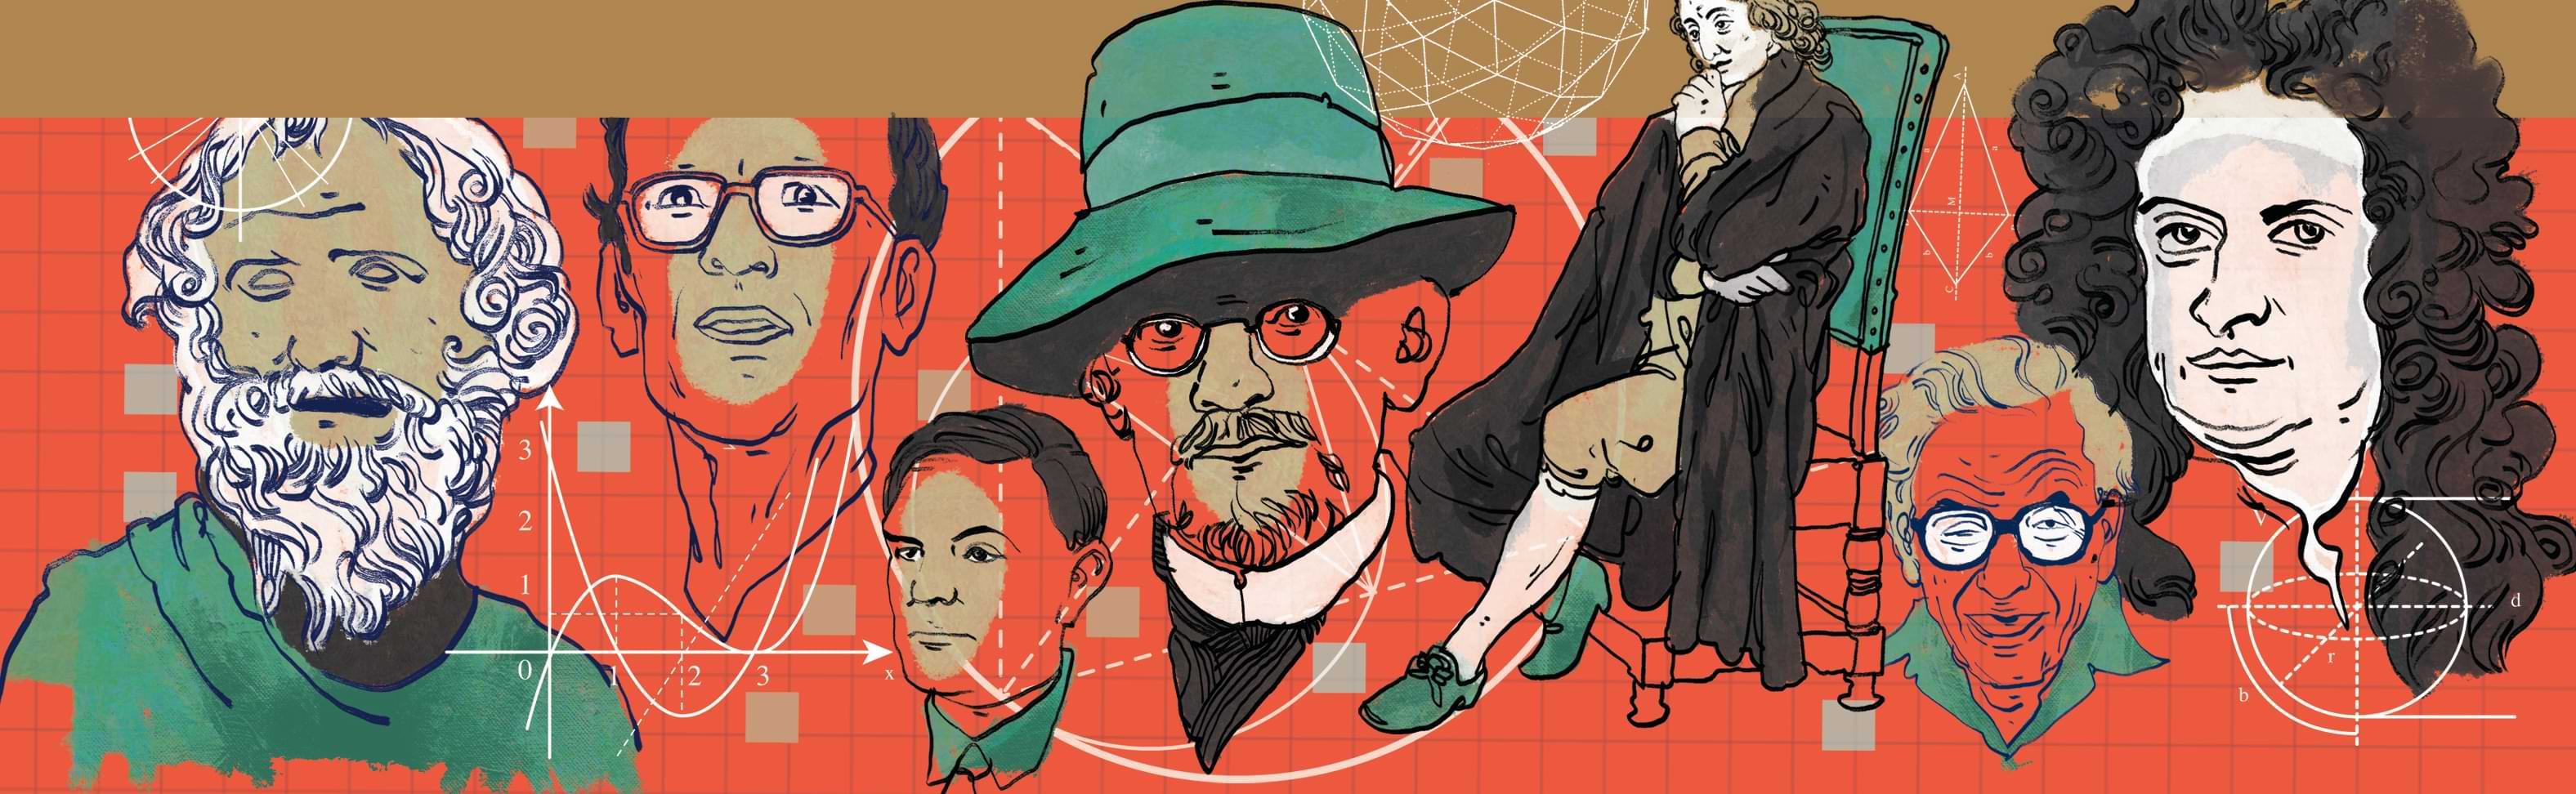
\includegraphics[width=19.3cm]{../bannerlichsu}}}
\AddToShipoutPicture*{\put(88,550){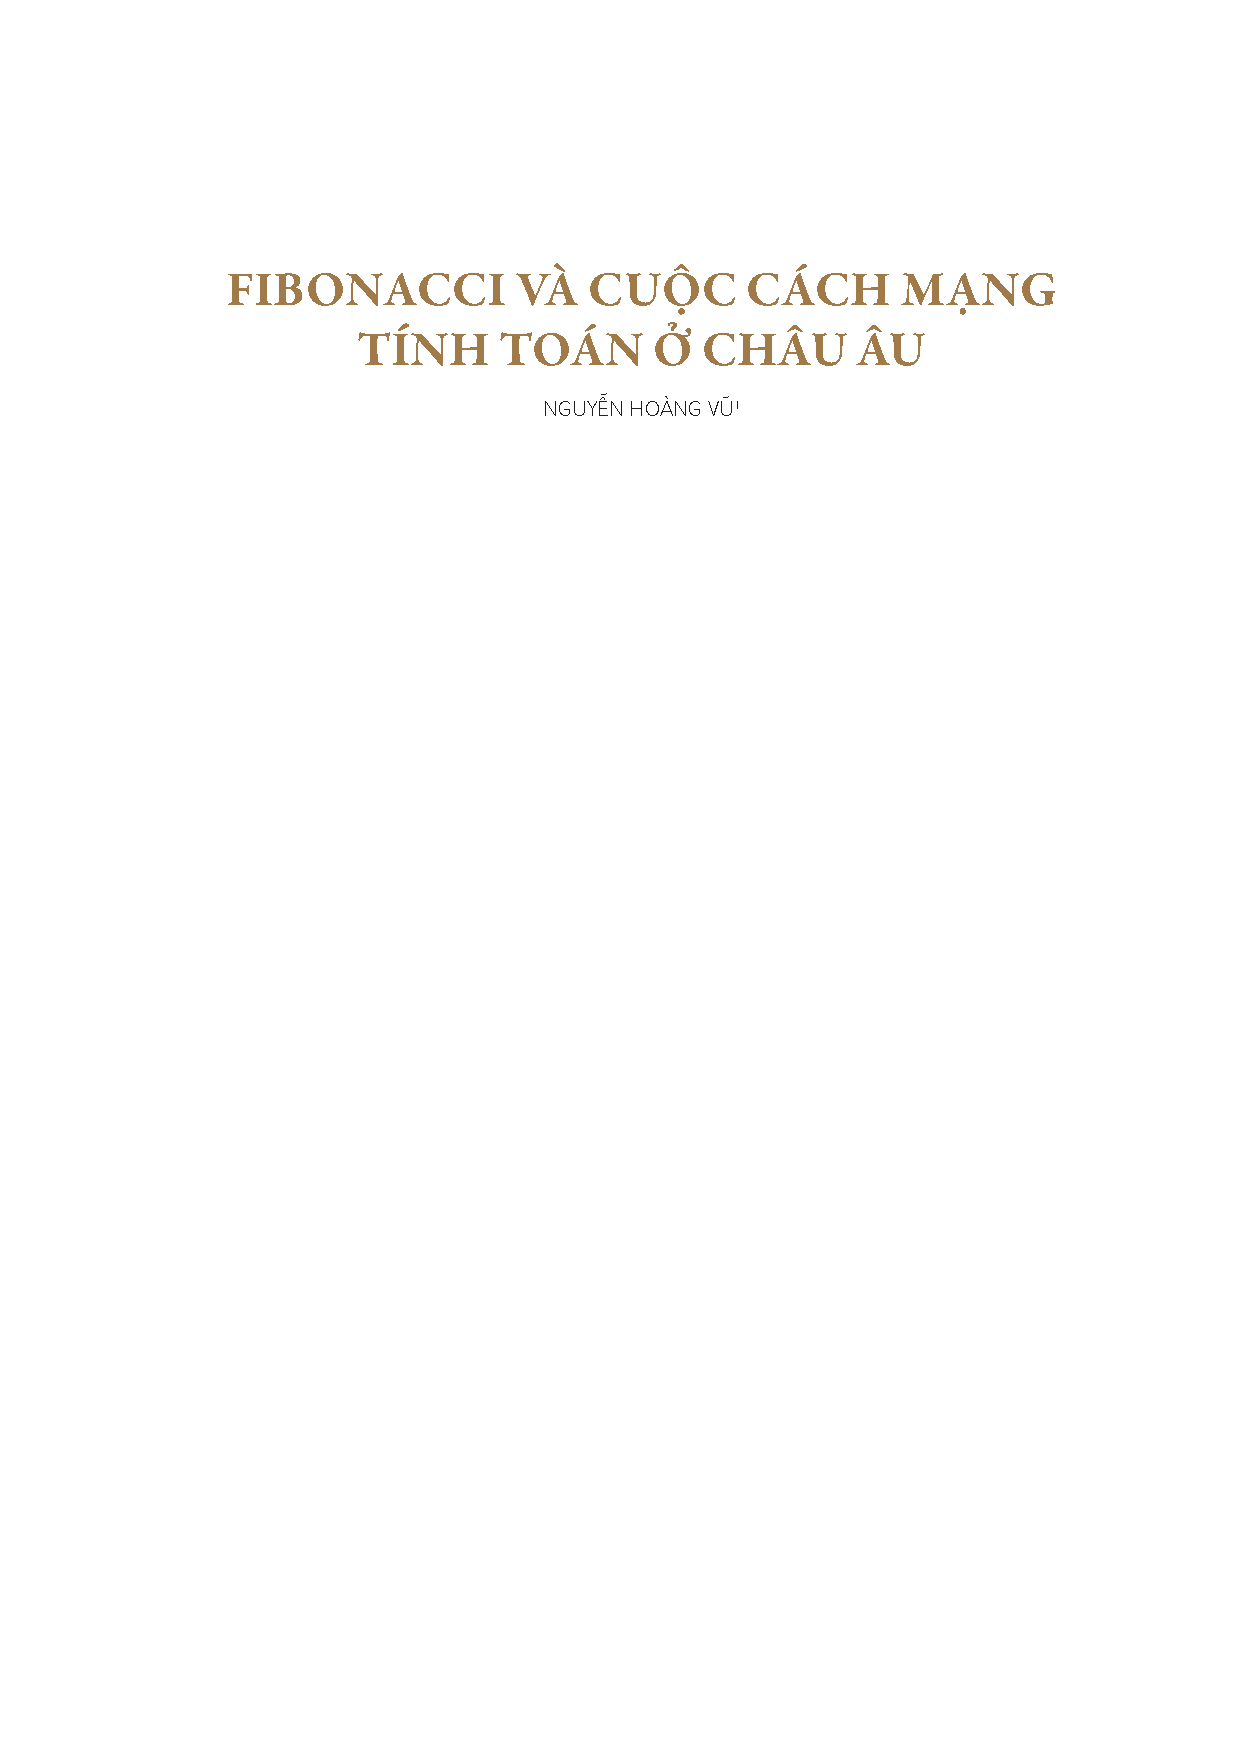
\includegraphics[scale=1]{../tieude2.pdf}}}
\centering
\endgroup

\vspace*{155pt}

\begin{multicols}{2}		
	Một ý tưởng tưởng chừng như mâu thuẫn với những cảm quan thường thức, thế nhưng lại trở thành một vũ trụ hình học mới lạ và chặt chẽ, và có thể nắm giữ bản chất của không gian chúng ta đang sống. Thế nhưng quá trình khám phá và phát triển ý tưởng ấy phải trải qua hàng thập kỷ với nhiều trắc trở và gian nan.
	\vskip 0.1cm
	\textbf{\color{lichsutoanhoc}Hy Lạp và Saccheri}
	\vskip 0.1cm
	Một trong những thứ mà người Hy Lạp cổ đại có thể tự hào với toàn thế giới chắc chắn là Toán học của họ, đặc biệt là Hình học phát triển bậc nhất nhân loại đương thời. Không chỉ những tính toán và đo đạc của họ có độ chính xác cao, hệ thống lý thuyết Hình học của họ cũng được thiết lập hết sức chặt chẽ, một điều hiếm thấy ở các nền văn minh đương thời. Minh chứng rõ ràng nhất chính là bộ ``Elements of Geometry" hay ``Elements" (Cơ sở) của Euclid thành Alexandria. Tác phẩm là một bản tổng hợp các kiến thức tự cổ chí kim của nền Hình học Hy Lạp đồ sộ, được sắp xếp theo trình tự khoa học, và quan trọng nhất: có sự xuất hiện của tiên đề, một số ít các mệnh đề được thừa nhận, để các kết quả sau đó được phát triển chỉ dựa trên những tiên đề ấy. Dù lý luận chưa kín kẽ hoàn toàn, một số chứng minh vẫn còn những điều được ngầm thừa nhận và một số vẫn phụ thuộc vào hình vẽ, và các tiên đề vẫn chưa đầy đủ (về sau ta sẽ chỉ ra những lỗi này) ``Elements" vẫn là một tác phẩm để đời của nhà sư phạm lỗi lạc. 
	\begin{figure}[H]
		\vspace*{-5pt}
		\centering
		\captionsetup{labelformat= empty, justification=centering}
		\includegraphics[width= 1\linewidth]{Sir_Henry_Billingsley's_first_English_version_of_Euclid's_Elements,_1570.png}
		%		\caption{\small\textit{\color{}}}
		\vspace*{-15pt}
	\end{figure}
	Ngoài việc Hình học được đặt trên nền móng logic như trên, đã có hẳn một phái nghiên cứu những ý nghĩa huyền bí của nó, đứng đầu bởi không ai khác ngoài Pythagoras xứ Samos. Trong số những giáo lý của triết gia bí ẩn này tới các môn đồ, Toán học giữ một vai trò cực kỳ quan trọng trong mục đích hàng đầu của họ -- hiểu thêm về thực tại và triết lý. Những con số (với phái này ``số" là các số nguyên dương khác $1$) được cho là ẩn chứa những lời giải thích về bản chất của vũ trụ, từ đó dẫn đến cách mô tả đậm chất Thần số học của họ. Hình học Euclid lại được coi là mô tả chính xác cho không gian thực. Quan điểm này sẽ trở thành niềm tin chủ đạo của giới học thuật châu Âu, do sự tiếp thu tri thức từ Hy Lạp cổ đại.
	\vskip 0.1cm
	Quay lại với Euclid, các tiên đề ông đưa ra sẽ là trọng tâm của chúng ta trong phần tới, đặc biệt là tiên đề cuối. Chúng lần lượt là:
	\vskip 0.1cm
	$1.$ Qua hai điểm bất kì, luôn luôn vẽ được một đường thẳng.
	\vskip 0.1cm
	$2.$ Có thể kéo dài một đoạn thẳng một đoạn dài hữu hạn theo hai hướng.
	\vskip 0.1cm
	$3.$ Với một điểm và một đoạn bất kỳ, luôn luôn vẽ được một đường tròn có tâm và bán kính lần lượt là điểm và có độ dài bằng đoạn đã nêu. 
	\vskip 0.1cm
	$4.$ Mọi góc vuông đều bằng nhau. Góc vuông được định nghĩa là góc bằng với góc bù của nó.
	\vskip 0.1cm
	$5.$ Nếu $2$ đường thẳng tạo với $1$ đường thẳng thứ $3$ hai góc trong cùng phía mà có tổng nhỏ hơn hai góc vuông thì chúng sẽ cắt nhau về phía đó, khi cả hai được kéo dài vô hạn.
	\vskip 0.1cm
	và $5$ định đề (common notion):
	\vskip 0.1cm
	$1.$ Hai cái cùng bằng cái thứ ba thì bằng nhau. 
	\vskip 0.1cm
	$2.$ Thêm những cái bằng nhau vào những cái bằng nhau thì được những cái bằng nhau.
	\vskip 0.1cm
	$3.$ Bớt đi những cái bằng nhau từ những cái bằng nhau thì được những cái bằng nhau.
	\vskip 0.1cm
	$4.$ Trùng nhau thì bằng nhau.
	\vskip 0.1cm
	$5.$ Toàn thể lớn hơn một phần.
	\vskip 0.1cm
	Trước khi đi tiếp, chúng ta cần hai kết quả đáng lưu tâm trong Elements ở đây:
	\vskip 0.1cm
	Định lý $16$ của ``Elements" Quyển I, tên khác là định lý góc ngoài, một dạng yếu hơn của định lý góc ngoài ta quen biết nhưng không cần tới tiên đề song song, khẳng định: 
	\vskip 0.1cm
	Trong một tam giác bất kỳ, góc ngoài của một đỉnh nào đó thì lớn hơn hai góc ở hai đỉnh còn lại.
	\vskip 0.1cm
	Khi thừa nhận thêm tiên đề $5$ thì góc ngoài sẽ bằng tổng hai góc ở hai đỉnh ấy luôn.
	\vskip 0.1cm
	Định lý $27$, định lý về góc so le trong: 
	\vskip 0.1cm
	Hai đường thẳng có một đường thứ ba cắt qua mà tạo với đường thứ ba hai góc so le trong bằng nhau thì là hai đường song song.
	\vskip 0.1cm
	Hai định lý này (cùng một số mệnh đề ngầm được thừa nhận) đã chỉ ra sự tồn tại của hai đường thẳng song song, và có thể được chứng minh mà không sử dụng tiên đề số $5$. Ba định đề đầu tiên còn đúng cả trong số học, trong khi định đề thứ $5$ có một câu chuyện riêng, ta để dành lúc khác. Nên nhớ rằng, theo cách hiểu được duy trì trong thời gian dài, một tiên đề là một sự thật tự nó hiển nhiên. 
	\vskip 0.1cm
	Không khó để thấy tiên đề cuối cùng trông phức tạp hơn nhiều so với những tiên đề còn lại. Nó được trình bày dưới dạng giả thiết -- kết luận, rồi còn chứa trong đó một giả sử hơi khó hình dung -- hai đường được kéo dài vô hạn, dù hành động này trên thực tế là không thể kiểm chứng. Vì thế không ít người đã nghi ngờ rằng đây thực chất là một định lý, và không ít trong số họ đã đổ thời gian và tâm sức vào nhằm đưa ra một chứng minh thỏa đáng. Hẳn rồi, nếu một trong các nỗ lực đó chính xác thì đã chẳng có bài viết này, tất cả đều không tránh được lỗi ngầm thừa nhận một khẳng định nào đó hóa ra lại tương đương với tiên đề $5$. Vậy là, kể từ khi thời Euclid, cho đến giai đoạn thất thoát sách vở Hy Lạp cổ đại, để rồi được những người Ả Rập tìm thấy và dựa vào đó đến phát triển, tới khi những lái buôn nơi đây đem Toán của mình tới châu Âu trong những cuộc giao thương, góp phần đánh thức nền Toán học chìm trong đêm dài Trung Cổ, cho tới mấy trăm năm ``Elements" làm cuốn sách hình học mẫu mực trên lục địa, sau bao nhiêu thế hệ trí thức chung tay giải quyết, thứ hậu thế thu được từ các chứng minh sai lầm hầu như chỉ là các phát biểu lại của tiên đề cuối cùng. 
	\vskip 0.1cm
	Điều này không có nghĩa là công sức của họ là vô ích hoàn toàn, ngược lại, đây là một sự chuẩn bị cần thiết cho những diễn biến tới. Hãy cùng điểm qua một vài phát biểu như vậy: 
	\vskip 0.1cm
	-- Playfair: Với một điểm $M$ không nằm trên một đường thẳng $d$ cho trước, qua $M$ có đúng $1$ đường thẳng song song với $d$. 
	\vskip 0.1cm 
	-- Định lý $30$ trong ``Elements": Nếu $3$ đường thẳng $a$, $b$, $c$ phân biệt và thỏa mãn: $a \parallel c$, $b \parallel c$, thì $a \parallel b$. Nói cách khác, quan hệ song song có tính bắc cầu.
	\vskip 0.1cm
	-- Farkas Bolyai: Luôn vẽ được một đường tròn đi qua cả $3$ đỉnh của một tam giác nào đó.
	\vskip 0.1cm
	-- Wallis: Tồn tại hai tam giác đồng dạng nhưng không bằng nhau.
	\vskip 0.1cm
	-- Tồn tại tam giác nào đó mà tổng ba góc của nó là hai góc vuông.
	\vskip 0.1cm
	-- Định lý Pytago: tổng diện tích hai hình vuông có cạnh là hai cạnh góc vuông của tam giác vuông bằng diện tích hình vuông có cạnh bằng cạnh huyền.
	\vskip 0.1cm
	-- Diện tích của tam giác không bị chặn.
	\vskip 0.1cm
	-- Góc nội tiếp chắn đường kính của đường tròn là góc vuông.
	\vskip 0.1cm
	-- Cho tứ giác $ABCD$ có các góc đỉnh $A$, $B$, $C$ là $3$ góc vuông, đây được gọi là một tứ giác Lambert. Khi ấy góc ở đỉnh $D$ cũng vuông.
	\vskip 0.1cm
	-- Cho tứ giác $ABCD: AB = CD$ và các góc đỉnh $B$, $C$ vuông. Ta gọi đây là một tứ giác Saccheri. Khi ấy góc đỉnh $A$ và đỉnh $D$ cũng vuông. Một phát biểu tương tự: hình chữ nhật có tồn tại.
	\vskip 0.1cm
	Cách phát biểu đầu tiên là dạng được trình bày trong sách giáo khoa, được đặt tên theo Playfair ($1748-1819$), một giáo sư Toán tại Đại học Edinburgh, dù nó được nghiên cứu bởi Proclus từ tận những năm $400$ TCN. Ta trình bày một chứng minh ngắn ở đây:
	\begin{figure}[H]
		\vspace*{-5pt}
		\centering
		\captionsetup{labelformat= empty, justification=centering}
		\definecolor{qqwuqq}{rgb}{0.,0.39215686274509803,0.}
		\definecolor{uuuuuu}{rgb}{0.26666666666666666,0.26666666666666666,0.26666666666666666}
		\begin{tikzpicture}[lichsutoanhoc]
			\draw [shift={(0.07058823529411783,4.)},color=qqwuqq,fill=qqwuqq,fill opacity=0.10000000149011612] (0,0) -- (-108.5792703804447:0.42) arc (-108.5792703804447:0.:0.42) -- cycle;
			\draw  (-2.,4.)-- (4.,4.);
			\draw  (-2.,1.)-- (4.,1.);
			\draw  (0.4,4.98)-- (-1.2,0.22);
			\draw  (-1.68,4.68)-- (4.02,2.44);
			\draw (2.7,4.37) node {$l''$};
			\draw (2.5,0.81) node {$l$};
			\draw (-0.72,2.37) node {$t$};
			\draw (2.64,3.39) node {$l'$};
			\draw [fill=white] (0.07058823529411783,4.) circle (1.5pt);
			\draw (0.,4.37) node {$P$};
			\draw [fill=white] (-0.9378151260504201,1.) circle (1.5pt);
			\draw (-0.78,0.71) node {$Q$};
		\end{tikzpicture}
		\vspace*{-10pt}
	\end{figure}
	Chứng minh: 
	(Playfair $\to$ Euclid)
	Gọi $t$ là đường thẳng cắt cả hai đường thẳng $l$ và $l'$ cho trước. $t$ cắt $l$ tại $Q$, cắt $l'$ tại $P$, hình thành hai góc trong cùng phía $g_1$ và $g_2$. Không mất tính tổng quát, giả sử $g_1 + g_2$ nhỏ hơn tổng độ lớn hai góc vuông.
	\vskip 0.1cm
	Nếu ta đặt $g_3$ là góc bù của $g_2$, khác phía với $g_1$ và $g_2$, thì $g_3 + g_2 = 180 > g_1 + g_2$, dẫn đến $g_1 < g_3$. Qua $P$, kẻ đường thẳng $l''$ tạo với $t$ một góc bằng và so le trong với $g_3$. Do $g_3 > g_1$, hai đường thẳng $l'$ và $l''$ là hai đường thẳng phân biệt. Theo tiên đề Playfair, $l'$ không thể song song với $l$, và phải cắt $l$ tại một điểm hữu hạn $R$ nào đó. Nếu $R$ nằm khác phía với $g_1$ và $g_2$, thì $g_1$ là một góc ngoài của tam giác $PQR$. Theo định lý góc ngoài, $g_1$ sẽ lớn hơn $g_3$, điều này vô lý. Do đó $R$ nằm cùng phía với $g_1$ và $g_2$, chứng minh được rằng tiên đề Playfair suy ra tiên đề song song.
	\vskip 0.1cm
	Trong những cuộc tấn công không ngớt vào bài toán chứng minh tiên đề thứ $5$, lịch sử đã đáng tiếc bỏ quên một công trình kỳ thú: Euclides ab omni naevo vindicatus (``Bào chữa cho mọi lỗi lầm của Euclid") của Girolamo Saccheri ($1667-1733$), một linh mục dòng Tên kiêm giáo sư tại đại học Pavia, Ý. 
	\vskip 0.1cm
	Saccheri được sinh vào ngày $5$ tháng $9$ năm $1667$, ở San Remo, Ý, thuộc quyền kiểm soát của Genoa vào thời ấy. Năm $1865$, khi lên 18 tuổi, ông tham gia Hội Tu sĩ Dòng Tên, và năm năm sau ông đến Milan để theo học triết học và thần học ở Brera, một đại học Dòng Tên. Tomasso Ceva, em trai của Giovanni Ceva (người có định lý nổi tiếng mang tên ông), đang là một giáo sư toán học ở đó, và khuyến khích Saccheri theo đuổi ngành học này.
	\vskip 0.1cm
	Saccheri nhắm tới việc chứng tỏ rằng tiên đề thứ $5$ thực chất là định lý, từ đó dập tắt chỉ trích của Ngài Henry Savile rằng tiên đề này là một ``sai lầm" của hình học. Phương pháp ông sử dụng cũng là một kỹ thuật nổi bật Euclid áp dụng -- reductio ad absurdum, cụm từ tiếng Latinh mang nghĩa ``phản chứng". Ông tiếp cận nó theo cách nhìn của phát biểu tương đương cuối cùng trong danh sách trên: Cho tứ giác ABCD với $AD = BC$ và các góc đỉnh $A$, $B$ vuông. Khi ấy góc đỉnh $C$ cũng vuông. Người ta gọi nó là giả thiết góc vuông. 
	Tứ giác Saccheri đã được nghiên cứu từ tận thế kỷ $12$ bởi nhà thơ kiêm nhà toán học người Iran Omar Khayyam, vào thế kỷ $13$ bởi nhà thiên văn học kiêm nhà toán học Nassir Adin trong một công trình có mục đích như của Saccheri, và về sau bởi một số học giả châu Âu như Clavius và Giordano Vitale. Tất nhiên tâm điểm nằm ở vị mục sư do ông đã phát triển xa hơn các tiền nhân nhiều.
	Không sử dụng tiên đề song song, ta chứng minh được hai góc đỉnh $C$ và $D$ bằng nhau (Saccheri $1$) như sau:
	\begin{figure}[H]
		\vspace*{-5pt}
		\centering
		\captionsetup{labelformat= empty, justification=centering}
		\begin{tikzpicture}[lichsutoanhoc]
			\draw (0,0) rectangle (6,3);
			\draw [fill=white] (0,0) circle (1.5pt) node[left] {$A$};
			\draw [fill=white] (0,3) circle (1.5pt) node[left] {$D$};
			\draw [fill=white] (6,0) circle (1.5pt) node[right] {$B$};
			\draw [fill=white] (6,3) circle (1.5pt) node[right] {$C$};
		\end{tikzpicture}
		\vspace*{-10pt}
	\end{figure}
	$\Delta BAD = \Delta ABC$ (c.g.c) vì $AD = BC$, $BAD = ABC = 90^\circ$, và chung $AB$. Khi đó ta có $BD = AC$. Từ đây ta suy ra $\Delta ADC = \Delta BCD$ (c--c--c). Từ đây ta có $2$ góc đỉnh $C$ và $D$ bằng nhau.
	\vskip 0.1cm
	Saccheri quyết định giả sử phản chứng rằng hai góc $C$ và $D$ không phải góc vuông, từ đó cho ra hai trường hợp:
	\vskip 0.1cm
	-- $C$ và $D$ là hai góc tù (giả thuyết góc tù).
	\vskip 0.1cm
	-- $C$ và $D$ là hai góc nhọn (giả thuyết góc nhọn).
	\vskip 0.1cm
	Đầu tiên ông chứng minh: nếu một trong hai giả thuyết này đúng với một tứ giác Saccheri nào đó, thì nó đúng với mọi tứ giác Saccheri. Sau đó ông chứng minh rằng giả thuyết góc tù sẽ dẫn đến tổng ba góc trong một tam giác bất kỳ là lớn hơn hai góc vuông, và ngược lại, giả thuyết góc nhọn sẽ dẫn đến tổng ba góc trong một tam giác bất kỳ nhỏ hơn hai góc vuông. 
	\begin{figure}[H]
		\vspace*{-5pt}
		\centering
		\captionsetup{labelformat= empty, justification=centering}
		\definecolor{qqwuqq}{rgb}{0.,0.39215686274509803,0.}
		\definecolor{uuuuuu}{rgb}{0.26666666666666666,0.26666666666666666,0.26666666666666666}
		\definecolor{ududff}{rgb}{0.30196078431372547,0.30196078431372547,1.}
		\begin{tikzpicture}[scale=1.2,lichsutoanhoc]
			\draw[color=qqwuqq,fill=qqwuqq,fill opacity=0.10000000149011612] (1.7171572875253809,2.) -- (1.7171572875253809,1.7171572875253809) -- (2.,1.7171572875253809) -- (2.,2.) -- cycle; 
			\draw[color=qqwuqq,fill=qqwuqq,fill opacity=0.10000000149011612] (-1.,2.282842712474619) -- (-1.2828427124746191,2.282842712474619) -- (-1.2828427124746191,2.) -- (-1.,2.) -- cycle; 
			\draw[color=qqwuqq,fill=qqwuqq,fill opacity=0.10000000149011612] (-3.,1.7171572875253809) -- (-2.717157287525381,1.7171572875253809) -- (-2.717157287525381,2.) -- (-3.,2.) -- cycle; 
			\draw  (-1.,4.)-- (-3.,0.);
			\draw  (-3.,0.)-- (2.,0.);
			\draw  (2.,0.)-- (-1.,4.);
			\draw  (-1.,4.)-- (-1.,2.);
			\draw  (-3.,0.)-- (-3.,2.);
			\draw  (2.,0.)-- (2.,2.);
			\draw  (2.,2.)-- (-3.,2.);
			\draw [fill = white] (-1.,4.) circle (1.5pt);
			\draw (-0.86,4.37) node {$A$};
			\draw [fill = white] (-3.,0.) circle (1.5pt);
			\draw (-3.06,-0.33) node {$B$};
			\draw [fill = white] (2.,0.) circle (1.5pt);
			\draw (1.92,-0.27) node {$C$};
			\draw [fill=white] (-2.,2.) circle (1.5pt);
			\draw (-1.92,1.69) node {$M$};
			\draw [fill=white] (0.5,2.) circle (1.5pt);
			\draw (0.3,1.73) node {$N$};
			\draw [fill = white] (-1.,2.) circle (1.5pt);
			\draw (-0.9,1.69) node {$D$};
			\draw [fill = white] (-3.,2.) circle (1.5pt);
			\draw (-3.02,2.49) node {$E$};
			\draw [fill = white] (2.,2.) circle (1.5pt);
			\draw (2.04,2.47) node {$F$};
		\end{tikzpicture}
		\vspace*{-5pt}
	\end{figure}
	Thật vậy, với tam giác ABC bất kỳ, lấy $M$, $N$ là trung điểm $AB$, $AC$, và gọi $D$, $E$, $F$ lần lượt là hình chiếu của $A$, $B$, $C$ lên $MN$. Lúc ấy $ \Delta BEM = \Delta ADM$, và $\Delta ADN = \Delta CFN$. Khi đó ta có $BE = AD = CF$, và $\angle BEF = \angle CFE = 90$. Khi đó $EFCB$ là một tứ giác Saccheri vuông tại $E$ và $F$. Qua cộng góc đơn giản ta chứng minh được tổng ba góc của tam giác chính là tổng hai góc $B$ và $C$ của tứ giác Saccheri $EFCB$.
	\vskip 0.1cm
	Từ bước chuẩn bị này, Saccheri đã bác bỏ giả thuyết góc tù bằng một chuỗi $13$ mệnh đề, rồi đến với kết luận sau cùng chính là tiên đề song song, một điều rõ ràng mâu thuẫn với giả sử giả thuyết góc tù đúng. Trích lời văn hoa mỹ của chính ông: ``Giả thuyết góc tù hoàn toàn sai bởi nó tự thủ tiêu chính nó".
	\vskip 0.1cm
	Giả thuyết góc nhọn lại là một câu chuyện khác hẳn. Saccheri đã chứng minh hết định lý này đến định lý khác, nhưng chẳng mâu thuẫn nào lộ diện. Các kết quả được chứng minh cứ thế chất chồng, dần dần hình thành một hệ thống phức tạp không hề thua kém so với hình học phẳng thông thường. Nhưng Saccheri, quá tin tưởng vào sứ mệnh của bản thân, đã để niềm tin sẵn có vào hình học Euclid gây rối mạch tư duy logic. Ông coi một điểm ở vô cùng như một điểm bình thường trên mặt phẳng, rồi ngộ nhận một cách đáng tiếc. 
	\vskip 0.1cm
	Gần với thời điểm xuất bản tác phẩm của Saccheri, chúng ta có những nghiên cứu của Lambert về loại tứ giác mang tên ông như nói ở trên. Tương tự như Saccheri, Lambert dễ dàng loại bỏ giả thuyết góc tù, và cũng chứng minh nhiều định lý với giả thuyết góc nhọn. Khác với Saccheri, Lambert nhận ra rõ ràng rằng mình không tiến đến một sự phi mâu thuẫn nào. Lambert không cho xuất bản những công trình về sau. 
	\vskip 0.1cm
	Tứ giác Saccheri có một tính chất không cần tới tiên đề $5$ như sau: đường nối trung điểm của $AB$ và $CD$ thì vuông góc với cả $AB$ và $CD$ (Saccheri $2$). Khi ấy ta thấy một tứ giác Saccheri đã được chia ra thành hai tứ giác Lambert. Do đó ta có thể chủ yếu nghiên cứu tính chất của tứ giác Saccheri ở đây.
	\begin{figure}[H]
		\vspace*{-5pt}
		\centering
		\captionsetup{labelformat= empty, justification=centering}
		\begin{tikzpicture}[scale=0.75,lichsutoanhoc]
			\draw (0,0) rectangle (8,4);
			\draw (0,4) -- (4,0) -- (8,4);
			\draw (4,0) -- (4,4);
			\draw [fill = white] (0,0) circle (2.0pt) node[left] {$A$};
			\draw [fill = white] (0,4) circle (2.0pt) node[left] {$D$};
			\draw [fill = white] (4,0) circle (2.0pt) node[below] {$E$};
			\draw [fill = white] (4,4) circle (2.0pt) node[above] {$F$};
			\draw [fill = white] (8,4) circle (2.0pt) node[right] {$C$};
			\draw [fill = white] (8,0) circle (2.0pt) node[right] {$B$};
		\end{tikzpicture}
		\vspace*{-10pt}
	\end{figure}
	Gọi $E$, $F$ lần lượt là trung điểm $AB$ và $CD$. Khi ấy $\Delta ADE = \Delta BCE$ (c.g.c), góc bằng nhau ở đỉnh $A$ và $B$. Từ đây có: $ \angle AED = \angle BEC, \angle ADE = \angle BCE, DE = CE$. Theo Saccheri $1$, $ \angle ADC = \angle BCD$, kết hợp lại ta được:
	\begin{align*}
		\angle EDF &= \angle EDC = \angle ADC - \angle ADE \\
		&= \angle BCD - \angle BCE \\
		&= \angle ECD = \angle ECF.
	\end{align*}
	Do đó $ \Delta DFE = \Delta CFE$ (c.g.c), suy ra $ \angle DFE = \angle CFE$. Hai góc này bù nhau nên chúng là góc vuông.
	Cũng có $ \angle DEF = \angle CEF$, cộng với $ \angle DEA = \angle CEB$ có $ \angle FEA = \angle FEB$, $ \angle FEA$ bằng với góc bù với nó nên là góc vuông nốt.
	\vskip 0.1cm
	Có thể thấy Saccheri đã hé mở cánh cửa tới một loại hình học nơi mà tiên đề song song bị bác bỏ, và dù ông đã hấp tấp đóng nó lại vì niềm tin vốn có, ý tưởng sử dụng phản chứng ông đưa ra là một bước tiến lớn. Trong số tiếp theo, chúng ta sẽ tìm hiểu quá trình khám phá của những người mở đường vào thế giới sau khe cửa hẹp đó. 
	\vskip 0.1cm
	\textbf{\color{lichsutoanhoc}Tài liệu tham khảo}
	\vskip 0.1cm
	-- Wikipedia tiếng Anh.
	\vskip 0.1cm
	-- Euclidean and Non--Euclidean Geometries -- Development and History (Marvin Jay Greenberg).
	\vskip 0.1cm
	-- Men of Mathematics The Lives and Achievements of the Great Mathematicians from Zeno to Poincaré (Eric Temple Bell).
	\vskip 0.1cm
	-- The History of Mathematics An Introduction (David M. Burton).
	\vskip 0.1cm
	-- https: //www.youtube.com/playlist?list=PL\\jLK2cYtt-VBSBtvfhxx-DW3Zw3nOQHVZ
	\vskip 0.1cm
	-- https: //rosetta.vn/lequanganh/wp-conten\\t/
	uploads/sites/7/2018/07/Riemann.pdf
	\vskip 0.1cm
	-- https: //www.cut-the-knot.org/triangle/py\\
	thpar/Drama.shtml
\end{multicols}

